\documentclass[conference]{IEEEtran}

% Pacotes essenciais para formatação, matemática, tabelas, código e imagens
\usepackage[utf8]{inputenc}
\usepackage[T1]{fontenc}
\usepackage[brazilian]{babel}
\usepackage{amsmath,amssymb,amsfonts}
\usepackage{algorithmic}
\usepackage{graphicx}
\usepackage{textcomp}
\usepackage{xcolor}
\usepackage{booktabs}
\usepackage{hyperref}
\usepackage{listings}
\usepackage{float}

% Configuração elegante para o código PLA e Verilog
\lstdefinestyle{codeStyle}{
  basicstyle=\ttfamily\footnotesize,
  frame=single,
  breaklines=true,
  columns=fullflexible,
  backgroundcolor=\color{gray!5},
  aboveskip=8pt,
  belowskip=8pt,
  xleftmargin=5pt,
  xrightmargin=5pt
}

\begin{document}

\title{Relatórios dos Laboratórios (Ciclo 2)}

\author{\IEEEauthorblockN{Francisco Passos dos Santos Alves}
\IEEEauthorblockA{\textit{Departamento de Computação} \\
\textit{Universidade Federal de Sergipe}\\
Aracaju, Sergipe, Brasil \\
email: francisco.alves@dcomp.ufs.br}

\and

\IEEEauthorblockN{João Vitor Vital Leão}
\IEEEauthorblockA{\textit{Departamento de Computação} \\
\textit{Universidade Federal de Sergipe}\\
Aracaju, Sergipe, Brasil \\
email: joao.leao2@dcomp.ufs.br}

\and

\IEEEauthorblockN{Lucca Pedreira Dultra}
\IEEEauthorblockA{\textit{Departamento de Computação} \\
\textit{Universidade Federal de Sergipe}\\
Aracaju, Sergipe, Brasil \\
email: lucca.dultra@dcomp.ufs.br}

\and 

\IEEEauthorblockN{Karlos Danyel Santos Gomes}
\IEEEauthorblockA{\textit{Departamento de Computação} \\
\textit{Universidade Federal de Sergipe}\\
Aracaju, Sergipe, Brasil \\
email: karlos.gomes2@dcomp.ufs.br}
}

\maketitle

\begin{abstract}
Este trabalho consolida as práticas do segundo ciclo da disciplina de Sistemas Digitais, propondo uma travessia completa pelos níveis de abstração do fluxo de projeto de circuitos integrados (VLSI). O estudo é dividido em três eixos metodológicos: (1) Nível Elétrico e Físico, através da simulação transiente de Standard Cells (Nangate 45nm) via NGSpice, quantificando o impacto do dimensionamento de transistores na dissipação de potência dinâmica e no consumo estático; (2) Nível Lógico, detalhando a implementação algorítmica do método de Quine-McCluskey em C++ para minimização booleana automatizada, utilizando padronização de arquivos PLA; e (3) Nível Arquitetural, onde topologias de somadores paralelos (Ripple Carry e Carry Lookahead) são sintetizadas em Linguagem de Descrição de Hardware (Verilog) no emulador Pitanga. Os resultados evidenciam os compromissos (trade-offs) indissociáveis entre área de silício, atraso de propagação e consumo energético, fornecendo uma visão holística e aprofundada dos desafios inerentes à microeletrônica moderna.
\end{abstract}

\begin{IEEEkeywords}
VLSI, NGSpice, Standard Cells, Quine-McCluskey, Verilog, Pitanga, CMOS, Dissipação de Potência, Carry Lookahead.
\end{IEEEkeywords}

% ==========================================
% SEÇÃO 1: INTRODUÇÃO
% ==========================================
\section{Introdução}
O avanço da Lei de Moore impulsionou a densidade de integração de transistores a níveis que desafiam a compreensão humana direta. Projetar um microprocessador contemporâneo, contendo bilhões de chaves semicondutoras, é uma tarefa viabilizada exclusivamente pelo uso de metodologias de abstração hierárquica e ferramentas de Automação de Projeto Eletrônico (EDA - \textit{Electronic Design Automation}).

O fluxo de projeto digital (\textit{Digital Design Flow}) moderno baseia-se na segregação do sistema em camadas. No nível inferior, as características físicas do silício — como resistências de canal, capacitâncias parasitas de difusão e correntes de fuga — ditam as limitações térmicas e de frequência do circuito. Nesse estrato, simuladores analógicos como o SPICE são ferramentas mandatórias para caracterizar \textit{Standard Cells} (células padrão industriais).

Subindo na hierarquia, equações lógicas complexas que descrevem o comportamento do sistema precisam ser otimizadas para reduzir a quantidade de portas físicas necessárias (minimização de área). Dado que métodos visuais (Mapas de Karnaugh) são ineficientes para mais de cinco variáveis, algoritmos matemáticos e determinísticos tornam-se o núcleo das ferramentas de síntese lógica.

Por fim, no nível de Transferência de Registradores (RTL), linguagens de descrição de hardware (HDLs) permitem aos engenheiros projetar a arquitetura estrutural de datapathes, como Unidades Lógicas e Aritméticas (ALUs), gerenciando os compromissos (\textit{trade-offs}) entre a velocidade computacional e a área de silício consumida. 

Este relatório documenta uma exploração extensiva dessas três camadas, integrando os Laboratórios 05 (Simulação SPICE), 06 (Quine-McCluskey em C++) e 07 (Síntese HDL em Verilog).

% ==========================================
% SEÇÃO 2: MATERIAIS E MÉTODOS
% ==========================================
\section{Materiais e Ambiente Experimental}
As práticas exigiram um conjunto diversificado de ferramentas de software, refletindo a pluralidade do fluxo EDA:
\begin{itemize}
    \item \textbf{Simulação de Baixo Nível (Lab 05):} NGSpice operando via interface de linha de comando. Utilizou-se o \textit{FreePDK45} (Predictive Technology Model) acoplado à biblioteca de células da Nangate para litografia de 45 nanômetros, operando sob uma tensão nominal $V_{DD} = 1.1\text{V}$.
    \item \textbf{Automação Algorítmica (Lab 06):} Ambiente de desenvolvimento C++ (compilador GCC). Manipulação de estruturas de dados nativas para leitura e escrita no formato matricial padronizado PLA (\textit{Programmable Logic Array}).
    \item \textbf{Síntese Digital e HDL (Lab 07):} Plataforma educacional Emulador Pitanga (InPlace). A modelagem foi inteiramente descrita utilizando o subconjunto sintetizável da linguagem Verilog.
\end{itemize}

% ==========================================
% SEÇÃO 3: LAB 05
% ==========================================
\section{Análise Física e Elétrica com \textit{Standard Cells} (Laboratório 05)}

O projeto baseado em Células Padrão (\textit{Standard Cells}) acelera o desenvolvimento de ASICs (Circuitos Integrados de Aplicação Específica) ocultando a geometria poligonal dos transistores sob uma interface de portas lógicas pré-caracterizadas. Contudo, o projetista precisa compreender o custo elétrico de suas escolhas lógicas.

\subsection{Simulação Transiente e Dimensionamento (Drive Strength)}
As bibliotecas fornecem a mesma porta lógica em diferentes dimensões, conhecidas como \textit{drive strengths} (ex: X1, X2, X4). O incremento deste índice implica no aumento da largura ($W$) do canal de condução dos transistores MOS internos. 

A primeira atividade consistiu em simular inversores (INV\_X1, INV\_X2, INV\_X4) e observar suas respostas temporais no NGSpice. Como evidenciado pela Figura \ref{fig1}, portas com maior \textit{drive} possuem menor resistência equivalente de condução ($R_{eq}$), o que lhes permite carregar a mesma capacitância de saída de forma substancialmente mais rápida (menor $t_{rise}$ e $t_{fall}$).

\begin{figure}[H]
\centerline{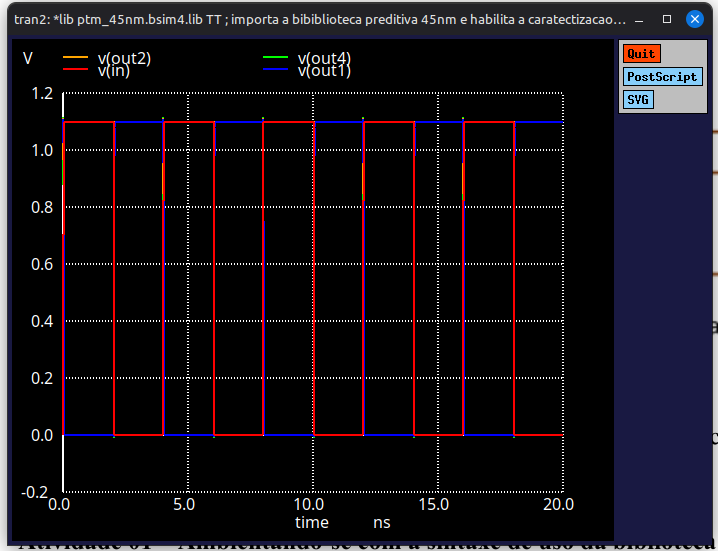
\includegraphics[width=\columnwidth]{1.png}}
\caption{Resposta transiente demonstrando as diferentes inclinações de chaveamento para inversores X1, X2 e X4.}
\label{fig1}
\end{figure}

\subsection{O Multiplexador 2:1 e a Potência Dinâmica}
Para extrair métricas de consumo quantitativas, instanciou-se um circuito Multiplexador 2:1 discreto composto por 1 porta NOT, 2 portas AND2 e 1 porta OR2 da biblioteca Nangate, todas inicialmente em tamanho base (\textbf{X1}). Uma carga $C_{load} = 10\text{fF}$ foi atrelada à saída. 

Os sinais de dados foram fixados em $\text{IN1} = 0\text{V}$ e $\text{IN2} = 1.1\text{V}$. A linha de seleção (\text{SEL}) operou com uma onda quadrada a 50 MHz. O comando transiente revelou que a corrente não flui constantemente; ela ocorre em espasmos agudos (Fig. \ref{fig2}).

\begin{figure}[H]
\centerline{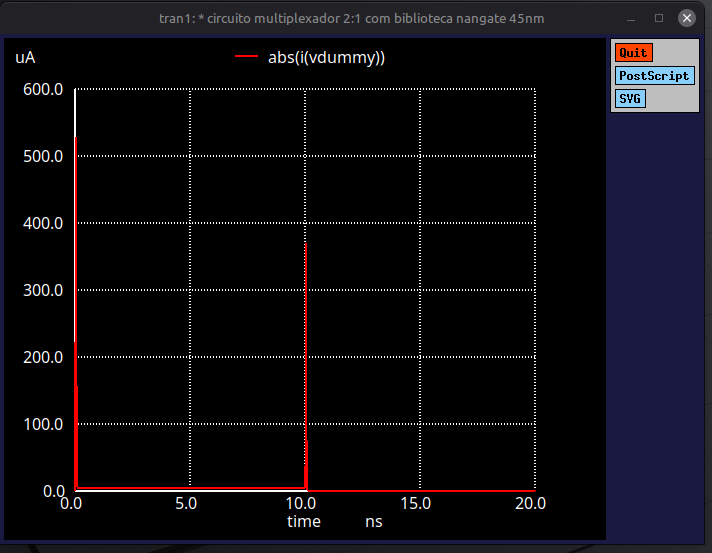
\includegraphics[width=\columnwidth]{2.png}}
\caption{Sinais de entrada, resposta da saída e a exata correlação temporal dos picos de corrente dinâmica com as transições de chaveamento.}
\label{fig2}
\end{figure}

A potência dinâmica em circuitos CMOS é matematicamente regida pela equação:
\begin{equation}
P_{din} = \alpha \cdot C_{total} \cdot V_{DD}^2 \cdot f
\end{equation}
onde $\alpha$ é o fator de atividade e $C_{total}$ engloba as cargas parasitas. Através da ferramenta de medição (\texttt{meas}) do NGSpice, obteve-se a corrente média ($I_{med}$) drenada da fonte para calcular a potência efetiva.

Para o MUX construído com células \textbf{1X}:
\begin{itemize}
    \item Corrente Média: $I_{med} = 3,91 \mu A$.
    \item $P_{1X} = 1.1\text{V} \times 3,91 \mu A = 4,30 \mu W$.
\end{itemize}

Para avaliar o custo do escalonamento, o código foi alterado substituindo-se todas as instâncias por suas contrapartes \textbf{2X}.
\begin{itemize}
    \item Corrente Média: $I_{med} = 9,77 \mu A$.
    \item $P_{2X} = 1.1\text{V} \times 9,77 \mu A = 10,75 \mu W$.
\end{itemize}

\begin{figure}[H]
\centerline{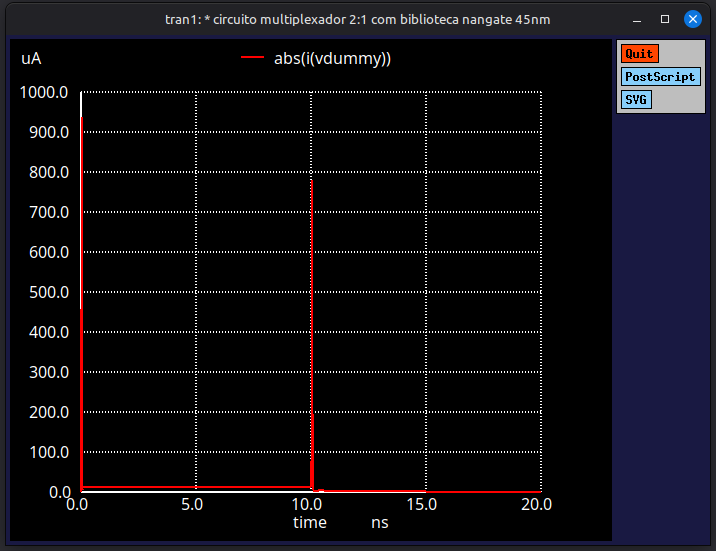
\includegraphics[width=\columnwidth]{3.png}}
\caption{Magnitude comparativa do pico de corrente gerado pela instância X2. O consumo mais que dobrou em relação ao MUX X1.}
\label{fig3}
\end{figure}

Este salto (maior que 100\%) na dissipação térmica comprova que portas mais "fortes" (X2, X4) aumentam não só o fornecimento de corrente, mas também a sua própria capacitância parasita interna devido ao aumento da área de Gate e de Difusão. Logo, projetistas de silício devem usar portas robustas apenas em caminhos críticos (\textit{critical paths}), sob pena de comprometer o \textit{budget} de energia do chip.

\subsection{Células Complexas e Consumo Estático (Leakage)}
A potência estática ocorre devido a fugas (\textit{leakage}) sub-limiares, mesmo quando a porta está em repouso. A investigação do \textit{datasheet} revelou que a célula complexa AND-OR-INVERT (\texttt{AOI21\_X1}) possui um \textit{leakage} drasticamente inferior à montagem equivalente com portas AND, OR e NOT separadas.

Essa discrepância deriva do leiaute planar. Na tecnologia CMOS, transistores dispostos em série (como na rede \textit{pull-down} de portas combinadas) podem compartilhar inteiramente as ilhas de difusão N+ (fonte de um conectada ao dreno de outro sem metalização intermediária). Ao eliminar junções, a célula \texttt{AOI} reduz a área e suprime caminhos de fuga pelo substrato, provando sua superioridade arquitetônica.

% ==========================================
% SEÇÃO 4: LAB 06
% ==========================================
\section{Otimização Lógica Computacional (Laboratório 06)}

A minimização de equações lógicas impacta diretamente na redução da área total do silício evidenciada na Seção 3. Como a inspeção visual por Mapas de Karnaugh é humana e falha, o algoritmo tabular proposto por W.V. Quine (1952) e refinado por E.J. McCluskey (1956) fornece a fundação da síntese automática.

\subsection{Mecânica do Algoritmo}
A implementação estruturada em C++ baseia-se em três etapas computacionais densas:
\begin{enumerate}
    \item \textbf{Agrupamento por Índices:} Os mintermos são convertidos para binário e agrupados conforme o peso de Hamming (quantidade de bits '1').
    \item \textbf{Combinação Exhaustiva:} Termos com diferença de peso igual a 1 são comparados (XOR). Se diferirem em exatamente um bit, fundem-se em um novo implicante, onde a discrepância é substituída pelo símbolo de \textit{Don't Care} ('-'). O processo é recursivo até atingir os Implicantes Primos.
    \item \textbf{Cobertura (Prime Implicant Chart):} Constrói-se uma matriz onde colunas são os mintermos originais e linhas os implicantes primos. O software identifica os \textit{implicantes primos essenciais} (únicos a cobrir determinado mintermo) e, se necessário, aplica heurísticas gulosas para cobrir os termos residuais.
\end{enumerate}

\subsection{Integração via Formato PLA}
Para comunicação nativa com outras ferramentas de EDA, o software manipula matrizes PLA (\textit{Programmable Logic Array}). Um exemplo prático foi o teste com uma função de 4 variáveis com os mintermos ativos: 0, 4 e 8.

\noindent\textbf{Arquivo de Entrada (\texttt{input.pla}):}
\begin{lstlisting}[style=codeStyle]
.i 4
.o 1
0000 1
0100 1
1000 1
.e
\end{lstlisting}

O software combinou os mintermos 0 e 4 gerando $0-00$; e os mintermos 0 e 8 gerando $-000$.

\noindent\textbf{Saída Automática (\texttt{result.pla}):}
\begin{lstlisting}[style=codeStyle]
F = A'C'D' + B'C'D'

.i 4
.o 1
0-00 1
-000 1
.e
\end{lstlisting}

A saída confirma que, ao invés de três portas AND de 4 entradas, o sintetizador precisará alocar apenas duas portas AND de 3 entradas, eliminando dependências lógicas. O código-fonte integral repousa no repositório GitHub do projeto.

% ==========================================
% SEÇÃO 5: LAB 07
% ==========================================
\section{Arquitetura e Síntese em HDL (Laboratório 07)}

Elevando a abstração, o Lab 07 lidou com a descrição estrutural e análise de datapathes aritméticos na linguagem Verilog, utilizando o Emulador Pitanga. O objeto de estudo foi a construção de somadores binários, bloco central de qualquer ALU.

\subsection{O Somador Completo Unitário (Full Adder)}
O FA de 1 bit recebe as parcelas $A_i, B_i$ e um transporte de entrada $C_{in}$, gerando a soma $S_i$ e o transporte de saída $C_{out}$. As equações implementadas na camada estrutural do Verilog são as clássicas:
\begin{align}
S_i &= A_i \oplus B_i \oplus C_{in} \\
C_{out} &= (A_i \cdot B_i) + (A_i \oplus B_i) \cdot C_{in}
\end{align}

\subsection{Expansão de Palavra (Ripple Carry Adder)}
A topologia RCA cascateia blocos FA sucessivos (4 bits, $N=4$). O pino $C_{out}$ do bit 0 liga-se ao $C_{in}$ do bit 1, e assim por diante. 

Embora estruturalmente trivial, o RCA sofre severamente com o tempo de propagação do sinal (\textit{critical path}). O cálculo final do bit $S_3$ só é computado após a cascata de três transportes anteriores ("vai-um") ter se estabilizado. O atraso cresce linearmente em função de $N$ ($O(N)$), inviabilizando microprocessadores de alto desempenho.

\subsection{Otimização de Latência (Carry Lookahead Adder)}
Para romper o atraso linear, implementou-se em Verilog a arquitetura CLA, que "antecipa" a presença de transportes achatando a malha booleana. Define-se:
\begin{itemize}
    \item Geração de Carry ($G_i$): $G_i = A_i \cdot B_i$ (Gera transporte independente do anterior).
    \item Propagação de Carry ($P_i$): $P_i = A_i \oplus B_i$ (Propaga se houver transporte anterior).
\end{itemize}

O transporte de qualquer estágio passa a ser modelado por uma árvore lógica paralela expansiva:
\begin{align}
C_1 &= G_0 + P_0 C_0 \\
C_2 &= G_1 + P_1 G_0 + P_1 P_0 C_0 \\
C_3 &= G_2 + P_2 G_1 + P_2 P_1 G_0 + P_2 P_1 P_0 C_0
\end{align}
Essa abordagem garante que todos os $C_{out}$ sejam calculados quase simultaneamente (apenas dois níveis lógicos de atraso, AND e OR).

\subsection{Análise do Trade-off de Síntese}
Os códigos foram submetidos ao sintetizador do Pitanga. A ferramenta mapeou o RTL para transistores básicos, expondo o clássico \textit{Trade-off} (Compromisso) entre Área e Velocidade (Tabela \ref{tab1}).

\begin{table}[H]
\caption{Comparativo de Síntese Lógica de Somadores (4 Bits)}
\begin{center}
\begin{tabular}{@{}lcc@{}}
\toprule
\textbf{Topologia Analisada} & \textbf{Transistores Utilizados} & \textbf{Área Ocupada (\%)} \\
\midrule
Ripple Carry Adder (RCA)      & 168                              & 1,68\%                     \\
Carry Lookahead Adder (CLA)   & 286                              & 2,86\%                     \\
\bottomrule
\end{tabular}
\label{tab1}
\end{center}
\end{table}

A compilação prova a restrição física do hardware. O RCA consumiu exatos 168 transistores, uma proporção estritamente linear (4 vezes os 42 transistores de um único FA). Contudo, a arquitetura CLA, projetada para contornar o atraso da malha, cobrou um preço estrutural severo: 286 transistores. Esse acréscimo massivo de $\sim 70\%$ de área é consumido puramente pelos blocos de geração e propagação antecipada.

% ==========================================
% SEÇÃO 6: CONCLUSÃO
% ==========================================
\section{Conclusões Integradas}
O ciclo de práticas reportado demonstrou com sucesso a sinergia entre as variadas camadas que formam a engenharia de computadores.

No Laboratório 05, o rigor da simulação em SPICE revelou que as leis da termodinâmica governam o silício: aumentar o desempenho individual de portas lógicas atrai custos severos de potência dinâmica e áreas repletas de parasitas. Isso fundamenta a necessidade de um nível de abstração superior otimizado.

Foi exatamente o que o Laboratório 06 ofereceu. Ao automatizar o algoritmo de Quine-McCluskey, validou-se como o tratamento matemático abstrato das funções lógicas minimiza os mintermos, salvando os preciosos transistores (e por consequência, a energia estática) analisados anteriormente.

A síntese dessas lições transpareceu de maneira clara no Laboratório 07. A utilização do Verilog para construir os somadores RCA e CLA não foi um mero exercício de codificação, mas sim a manifestação empírica da tomada de decisão de alto nível. Comprovou-se numericamente (168 vs 286 transistores) que arquiteturas velozes consomem invariavelmente mais área. Portanto, projetar sistemas digitais eficientes é a arte de transitar entre a teoria de grafos lógicos e o comportamento capacitivo dos semicondutores, garantindo a performance arquitetural sob o orçamento térmico do invólucro.

\begin{thebibliography}{00}
\bibitem{b1} R. A. L. Reis, \textit{Concepção de Circuitos Integrados}. Porto Alegre: Bookman, 2009.
\bibitem{b2} J. P. Uyemura, \textit{Sistemas Digitais: Uma Abordagem Integrada}. São Paulo: Thomson/Pioneira, 2002.
\bibitem{b3} R. Tocci, N. Widmer, e G. Moss, \textit{Sistemas Digitais - Princípios e Aplicações}, 12ª ed. São Paulo: Pearson, 2018.
\bibitem{b4} E. J. McCluskey, ``Minimization of Boolean Functions,'' \textit{Bell System Technical Journal}, vol. 35, no. 6, pp. 1417--1444, 1956.
\bibitem{b5} Samir Palnitkar, \textit{Verilog HDL: A Guide to Digital Design and Synthesis}, 2ª ed. Prentice Hall, 2003.
\end{thebibliography}

\end{document}